\documentclass[a4paper,12pt]{article}
\usepackage[english]{babel}
\usepackage[utf8]{inputenc}

%
% For alternative styles, see the biblatex manual:
% http://mirrors.ctan.org/macros/latex/contrib/biblatex/doc/biblatex.pdf
%
% The 'verbose' family of styles produces full citations in footnotes, 
% with and a variety of options for ibidem abbreviations.
%
\usepackage{graphicx}
\usepackage{csquotes}
\usepackage[style=verbose-ibid,backend=bibtex]{biblatex}
\bibliography{sample}

\usepackage{lipsum} % for dummy text

\title{Safe Policy Improvement by Minimizing Robust Baseline Regret}

\author{Shayan Amani}

\date{\today}

\begin{document}
\maketitle

\section{Summary}
Safety is what you need to have at hand when you are trying to persuade stakeholders. As a matter of interest, ensuring about the model's performance is always favorable and in some cases essential. This paper tries to come up with a \textit{safe} policy which guarantees better performance than the \textit{baseline} policy. Authors explained how to go beyond regular robustness common in the literature with demonstrating proofs and proposing the algorithm. 

Regret minimization is a topic of interest in RL which is discussed fairly well in this paper. Performance-wise talking, the proposed approach is promising over other available methods. 

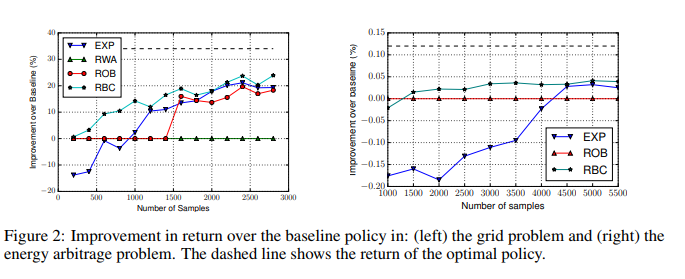
\includegraphics[width=1\columnwidth]{fig2.png}


\end{document}